\documentclass[10pt]{beamer}

\usetheme{metropolis}
\usepackage{appendixnumberbeamer}

\usepackage{booktabs}
\usepackage[scale=2]{ccicons}

\usepackage{pgfplots}
\usepgfplotslibrary{dateplot}

\usepackage{xspace}
\newcommand{\themename}{\textbf{\textsc{metropolis}}\xspace}

\usepackage{media9}

\usepackage{float}
\usepackage{subcaption}
\usepackage{epstopdf}

\usepackage{mathtools}
\newcommand{\conv}{\mathop{\bf conv}}
\usepackage{bm}

\usepackage{amsmath,amssymb}
\usepackage{amsthm}
% \newtheorem{theorem}{Theorem}

% \usepackage{marvosym}

% \let\theorem\relax
% \newtheorem{proposition}{Proposition}
% \newtheorem{definition}{Definition}
% \newtheorem{corollary}{Corollary}
% \newcommand\numberthis{\addtocounter{equation}{1}\tag{\theequation}}
% \DeclareMathOperator{\sign}{\text{sgn}}
% \DeclareMathOperator*{\argmin}{arg\,min}
% \DeclareMathOperator{\intr}{int}
% \DeclareMathOperator{\dom}{dom}
% \DeclareMathOperator{\rot}{\text{rot}}

\usepackage{tikz}
\usetikzlibrary{scopes}
\usetikzlibrary{shapes.misc}
\usetikzlibrary{shapes.arrows}
\tikzset{cross/.style={cross out, draw=black, minimum size=2*(#1-\pgflinewidth), inner sep=0pt, outer sep=0pt}, %default radius will be 1pt. 
cross/.default={2pt}}

\title{Exact Bounds on the Contact Driven Motion of a Sliding Object}
\subtitle{With Applications to Robotic Pulling}
\date{\today}
\author{Eric Huang$^1$, Ankit Bhatia$^2$, Byron Boots$^1$, Matt Mason$^2$}
\institute{$^1$Georgia Institute of Technology, $^2$Carnegie Mellon University}
% \titlegraphic{\hfill\includegraphics[height=1.5cm]{logo.pdf}}

\begin{document}

\maketitle

\begin{frame}{Table of contents}
  \setbeamertemplate{section in toc}[sections numbered]
  \tableofcontents[hideallsubsections]
\end{frame}

\section{Introduction}

\begin{frame}{Introduction}
  We explore the quasi-static motion of a planar slider being pushed
  through a non-slipping contact point.\vspace{3mm}

  Our main contributions are
  \begin{itemize}
  \item An algorithm that computes exact bounds on the object's
    motion
  \item An optimization-based planner that uses the exact bounds to
    plan convergent pulling trajectories
  \end{itemize}
\end{frame}

\section{Background}

\begin{frame}{Quasi-static Theory of Planar Pushing}
  % Theory
  \begin{columns}[c,onlytextwidth]
    \column{0.5\textwidth}

    \begin{list}{}{
        \setlength{\leftmargin}{0pt}
        \setlength{\labelwidth}{0pt}
        \setlength{\labelsep}{0pt}
      }
    \item%\<1->%\ 
      Twist: 
      \begin{equation*}
        \mathbf{v}^+ = [\mathbf{v}^T, \omega]^T
      \end{equation*}
    \item%<2-> 
      Body point velocity:
      \begin{equation*}
        A(\mathbf{x})\mathbf{v}^+ = 
        \begin{bmatrix*}[r]
          1 & 0 & -x_2 \\
          0 & 1 &  x_1
        \end{bmatrix*}\mathbf{v}^+
      \end{equation*}
    \item%<3-> 
      Total frictional moment:
      \begin{equation*}
        \mathbf{m}_f = -\mu\int_{R}\mathbf{r}\times\frac{A(\mathbf{r})\mathbf{v}^+}{\lVert A(\mathbf{r})\mathbf{v}^+ \rVert} p(\mathbf{r}) dA
      \end{equation*}
    \item%<4-> 
      Quasi-static assumption:
      \begin{equation*}
        \mathbf{m}_f = 0
      \end{equation*}
    \end{list}

    \column{0.5\textwidth}
    \begin{figure}
      \centering
      \def\iangle{35} % Angle of the inclined plane
      \begin{tikzpicture}[
        scale=1.25, every node/.style={scale=1.25},
        force/.style={>=latex,draw=black,fill=black},
        axis/.style={densely dashed,draw=gray,font=\small},
        ]
        \fill[draw=black,fill=blue!10,thin,rotate=\iangle] (-0.3,-0.5) rectangle (2.3,.5);
        \draw[rotate=\iangle] (1,0) circle[radius=2.4pt] node[cross] {};
        \draw[rotate=\iangle] (1,0) node[above right] {\tiny CoP};
        \draw [->,line width=1pt,rotate=-62.5] (0,0) ++(0,1) arc (90:30:1.0) node[right] {$\omega$};
        {[axis,->]
          \draw (0,0) -- (2.5,0) node[right] {$x$};
          \draw (0,0) -- (0,2.5) node[above] {$y$};
        }
        {[force,->]
          \draw (0,0) -- ++(0,1.5) node[right] {$\mathbf{v}$};
        }
        \fill (0,0) circle [radius=1.pt];
        % \fill (1.2207,0) circle [radius=1.pt] node[below right] {$x_{\text{\tiny IC}}$};

      \end{tikzpicture}
      % \caption{Motion of a press-pulled slider.}
      % \BB{Define variables and provide a short explanation of the figure.}}
      % \label{fig:presspull-motion}
    \end{figure}

  \end{columns}
\end{frame}

\begin{frame}{Quasi-static Theory of Planar Pushing}
  % Theory
  \begin{columns}[c,onlytextwidth]
    \column{0.5\textwidth}

    \begin{list}{}{
        \setlength{\leftmargin}{0pt}
        \setlength{\labelwidth}{0pt}
        \setlength{\labelsep}{0pt}
      }
    \item Principle of Minimal Dissipation:
    \item the motion $\mathbf{v}^+$ satisfies
      \begin{equation*} \begin{aligned}
          & \underset{\mathbf{v}^+}{\text{minimize}}
          & & \mu\int_R\lVert A(\mathbf{r})\mathbf{v}^+ \rVert p(\mathbf{r}) dA \\
          & \text{subject to}
          & & \mathbf{v}^+ \in \mathcal{C}.
        \end{aligned} \label{eq:constrained-frictional-dissipation}
      \end{equation*}
    \item where $\mathcal{C} = \{[0,1,\omega]^T, \omega \in \mathbb{R}\}$
    \end{list}\vspace{3.5mm}

    Is useful because
    \begin{itemize}
    \item cost continuous \& convex in $\mathbf{v}^+$
    \item $\equiv$ quasi-static assumption
    \end{itemize}

    \column{0.5\textwidth}
    \begin{figure}
      \centering
      \def\iangle{35} % Angle of the inclined plane
      \begin{tikzpicture}[
        scale=1.25, every node/.style={scale=1.25},
        force/.style={>=latex,draw=black,fill=black},
        axis/.style={densely dashed,draw=gray,font=\small},
        ]
        \fill[draw=black,fill=blue!10,thin,rotate=\iangle] (-0.3,-0.5) rectangle (2.3,.5);
        \draw[rotate=\iangle] (1,0) circle[radius=2.4pt] node[cross] {};
        \draw[rotate=\iangle] (1,0) node[above right] {\tiny CoP};
        \draw [->,line width=1pt,rotate=-62.5] (0,0) ++(0,1) arc (90:30:1.0) node[right] {$\omega$};
        {[axis,->]
          \draw (0,0) -- (2.5,0) node[right] {$x$};
          \draw (0,0) -- (0,2.5) node[above] {$y$};
        }
        {[force,->]
          \draw (0,0) -- ++(0,1.5) node[right] {$\mathbf{v}$};
        }
        \fill (0,0) circle [radius=1.pt];
        % \fill (1.2207,0) circle [radius=1.pt] node[below right] {$x_{\text{\tiny IC}}$};

      \end{tikzpicture}
      % \caption{Motion of a press-pulled slider.}
      % \BB{Define variables and provide a short explanation of the figure.}}
      % \label{fig:presspull-motion}
    \end{figure}

  \end{columns}
\end{frame}

\begin{frame}{Moment Envelope}
  \begin{columns}[c,onlytextwidth]
    \column{0.5\textwidth}
    % Given twist $\mathbf{v}^+$, region $R$ \textbf{(a)}
    \begin{itemize}%[<+->]
      \item[\textbf{(a)}] Given twist $\mathbf{v}^+$, region $R$
      \item[\textbf{(b)}] Torque from unit pressure at $\mathbf{r}$:
      \begin{equation*}
        g(\mathbf{r}) = -\mu\,\mathbf{r}\times \frac{A(\mathbf{r})\mathbf{v}^+}{\lVert A(\mathbf{r})\mathbf{v}^+ \rVert}
      \end{equation*}
      Moment surface function:
      \begin{equation*}
        G(\mathbf{r}) =
        \begin{bmatrix*}
          \mathbf{r}\\
          g(\mathbf{r})
        \end{bmatrix*}
      \end{equation*}
    \item[\textbf{(c)}] Moment envelope:
      \begin{equation*}
        \conv G(R)
      \end{equation*}
    \item[\textbf{(d)}] Feasible CoPs ($\mathbf{m}_f=0$):
      \begin{equation*}\conv G(R) \cap \{z=0\}\end{equation*}
    \end{itemize}

    \column{0.5\textwidth}
    \begin{figure}[t]
      \centering
      \begin{subfigure}[b]{0.49\textwidth}
        \centering
        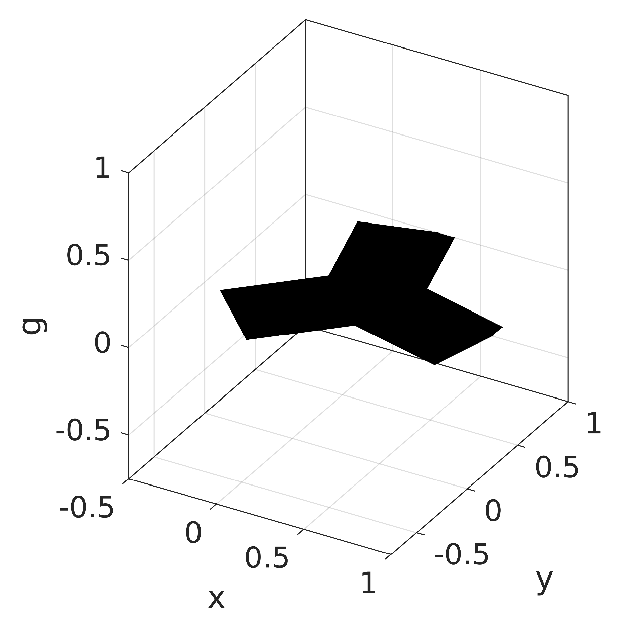
\includegraphics[width=1\linewidth]{./fig/moment_hull_1}
        \caption{}
      \end{subfigure}
      \begin{subfigure}[b]{0.49\textwidth}
        \centering
        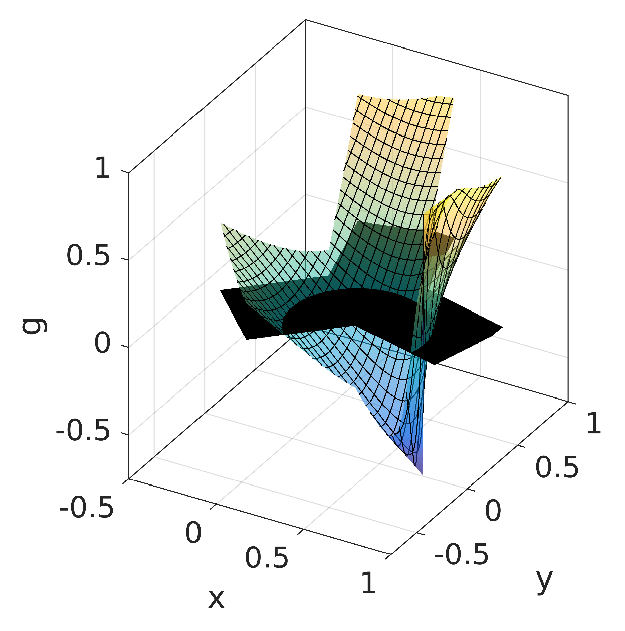
\includegraphics[width=1\linewidth]{fig/moment_hull_2}
        \caption{}
      \end{subfigure}
      \begin{subfigure}[b]{0.49\textwidth}
        \centering
        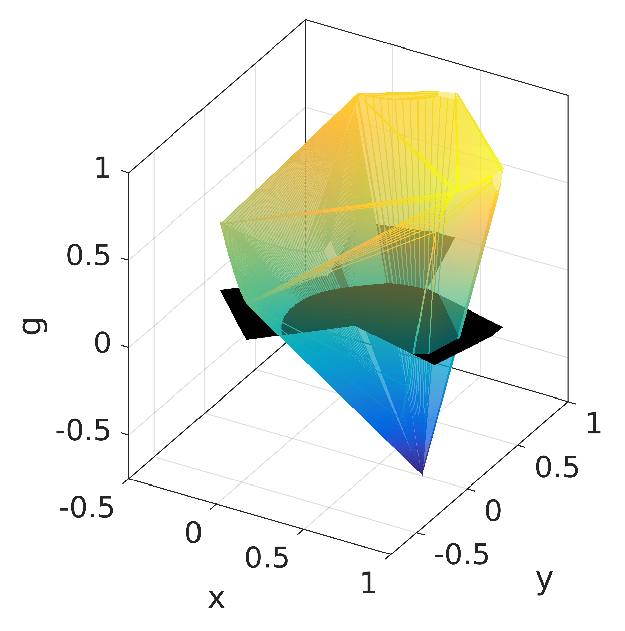
\includegraphics[width=1\linewidth]{fig/moment_hull_3}
        \caption{}
      \end{subfigure}
      \begin{subfigure}[b]{0.49\textwidth}
        \centering
        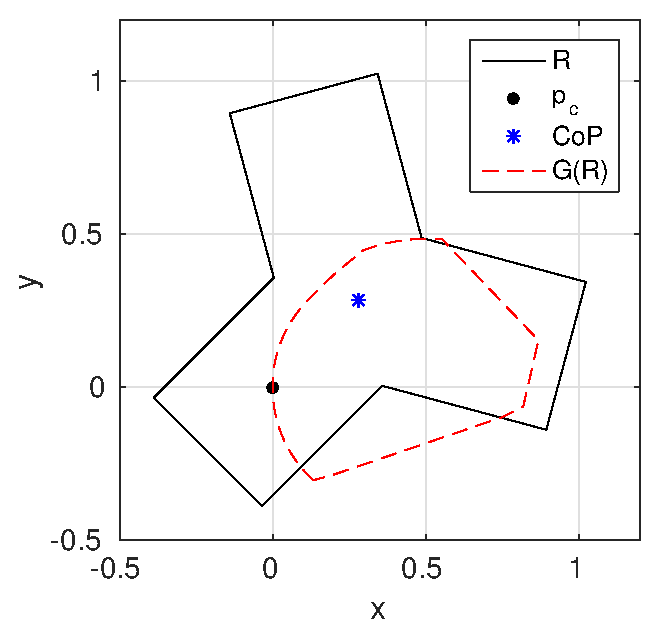
\includegraphics[width=1\linewidth]{fig/CoP_boundary}
        \caption{}
      \end{subfigure}
      % \caption{Example moment envelope for a trigonal 2D object with
      % rotation center $x_{\text{IC}} = 0.75$. (a) Support region
      % $R$. (b) Normalized-moment surface $G(R)$. (c) Convex moment
      % envelope of $G(R)$. (d) Intersection of the moment envelope and
      % the $xy$-plane. The intersection bounds the set of feasible
      % centers of pressure with zero moment.}
      % \label{fig:moment-envelope}
    \end{figure}
  \end{columns}
\end{frame}

\section{Theory}

\begin{frame}{Angular Velocity Bounds Properties}

  \begin{columns}[c,onlytextwidth]
    \column{0.5\textwidth}

    \begin{list}{}{
        \setlength{\leftmargin}{0pt}
        % % \settowidth{\leftmargini}{\usebeamertemplate{itemize item}}
        % % \addtolength{\leftmargini}{\labelsep}
        \setlength{\labelwidth}{0pt}
        \setlength{\labelsep}{0pt}
        % \setlength{\labelindent}{0pt}
        % \setlength{\itemindent}{0pt}
        % \setlength{\leftskip}{-\@totalleftmargin}
      }
    \item Fix $\theta$
    \item $\omega$ is \textit{feasible} if
      \begin{equation*}
      \mathbf{m}_f(\omega) = 0
      \end{equation*}
    \item Feasible set:
      \begin{equation*}
      \Omega = \{\omega\; |\; \mathbf{m}_f(\omega) = 0\}
      \end{equation*}
    \end{list}
    \begin{theorem}
      The feasible set $\Omega$ is connected and bounded.
    \end{theorem}

    % Bounds:
    \begin{align*}
      \alpha &= \max \Omega\\
      \beta &= \min \Omega
    \end{align*}

    \column{0.5\textwidth}

    \begin{figure}
      \centering
      \def\iangle{35} % Angle of the inclined plane
      \begin{tikzpicture}[
        scale=0.80, every node/.style={scale=0.75},
        force/.style={>=latex,draw=black,fill=black},
        axis/.style={densely dashed,draw=gray,font=\small},
        ]
        \fill[draw=black,fill=blue!10,thin,rotate=\iangle] (-0.3,-0.5) rectangle (2.3,.5);
        \draw[rotate=\iangle] (1,0) circle[radius=2.4pt] node[cross] {};
        \draw[rotate=\iangle] (1,0) node[above right] {\tiny CoP};
        \draw [rotate=-62.5] (0,0) ++(0,1) arc (90:30:1.0) node[right] {$\theta$};
        \draw [->,rotate=-120] (0,0) ++(0,1) arc (90:30:1.0);
        {[axis,->]
          \draw (-1,0) -- (2.5,0) node[right] {$x$};
          \draw (0,-1.5) -- (0,2.5) node[above] {$y$};
        }
        {[force,->]
          \draw (0,0) -- ++(0,1.5) node[right] {$\mathbf{v}$};
        }
        \fill (0,0) circle [radius=2.pt];
        % \fill (1.2207,0) circle [radius=1.pt] node[below right] {$x_{\text{\tiny IC}}$};

      \end{tikzpicture}
      % \caption{Motion of a press-pulled slider.}
      % \BB{Define variables and provide a short explanation of the figure.}}
      % \label{fig:presspull-motion}
    \end{figure}

    \begin{tikzpicture}
      \node[anchor=south west,inner sep=0] (image) at (0,0) {\includegraphics[width=\linewidth]{fig/omega_bounds_1}};
      \draw[line width=1.25] (2.3,2.34) -- ++(0,1.08) node[right] {$\Omega$};
      \definecolor{BLUE}{RGB}{0,113,188}
      \definecolor{ORANGE}{RGB}{216,82,24}
      \draw[line width=1.25,color=BLUE] (1.75,1.5) -- ++(0.25,0) node[right] {$\beta$};
      \draw[line width=1.25,color=ORANGE] (3.375,2.775) -- ++(0.25,0) node[right] {$\alpha$};
    \end{tikzpicture}

  \end{columns}
\end{frame}

\begin{frame}{Orientation Bounds}
    \begin{columns}[c,onlytextwidth]
    \column{0.5\textwidth}

    \begin{list}{}{
        \setlength{\leftmargin}{0pt}
        % % \settowidth{\leftmargini}{\usebeamertemplate{itemize item}}
        % % \addtolength{\leftmargini}{\labelsep}
        \setlength{\labelwidth}{0pt}
        \setlength{\labelsep}{0pt}
        % \setlength{\labelindent}{0pt}
        % \setlength{\itemindent}{0pt}
        % \setlength{\leftskip}{-\@totalleftmargin}
      }
    \item Contact point path:\vspace{-2mm}
      \begin{align*}
        &\gamma : \mathbb{R}\rightarrow\mathbb{R}^2, \quad \lVert\dot{\gamma}\rVert = 1\\
        &\rho = \tan^{-1}(\dot{\gamma}_y,\dot{\gamma}_x)
      \end{align*}
    \item Dynamics:\vspace{-2mm}
      \begin{align*}
        &\left.
        \begin{aligned}
          \dot{x} &= \cos(\rho)\\
          \dot{y} &= \sin(\rho)\\
          \dot{\varphi} &= \omega(\varphi - \rho + \pi)
        \end{aligned}\quad\right\}\quad\text{state}\\
        &\left.
        \begin{aligned}
        \dot{u} &=  \alpha(u - \rho + \pi) \\
        \dot{\ell} &=  \beta(\ell - \rho + \pi)
        \end{aligned}\quad\:\right\}\quad\text{bounds}
      \end{align*}
    \end{list}\vspace{-3mm}
    \begin{theorem}
      Given $\gamma$ and $\ell_0=\varphi_0=u_0$, then
      $\ell(t) \leq \varphi(t) \leq u(t), t \in [0,\infty)$
    \end{theorem}

    \column{0.5\textwidth}

    \begin{figure}
      \centering
      \def\iangle{-115} % Angle of the inclined plane
      \begin{tikzpicture}[
        scale=0.80, every node/.style={scale=0.75},
        force/.style={>=latex,draw=black,fill=black},
        axis/.style={densely dashed,draw=gray,font=\small},
        ]
        \fill[draw=black,fill=blue!10,thin,rotate=\iangle] (-0.3,-0.5) rectangle (2.3,.5);
        \draw[rotate=\iangle] (1,0) circle[radius=2.4pt] node[cross] {};
        \draw[rotate=\iangle] (1,0) node[below left] {\tiny CoP};

        % rho
        \def\rhol{0.50}
        \draw [rotate=0] (0,0) -- ++(\rhol,0) arc (0:130:\rhol) -- (0,0);
        \draw [dotted,rotate=0] (0,0) ++(\rhol,0) arc (0:50:\rhol) node[above right] {$\rho$};
        % varphi
        \def\phil{0.75}
        \draw [rotate=0] (0,0) -- ++(\phil,0) arc (0:-115:\phil) -- (0,0);
        \draw [rotate=0] (0,0) ++(\phil,0) arc (0:-30:\phil) node[right] {$\varphi$};
        % varphi - rho + pi
        \def\vrpl{1.}
        \draw [rotate=-50] (0,0) -- ++(\vrpl,0) arc (0:-65:\vrpl) -- (0,0);
        \draw [rotate=-50] (0,0) -- ++(\vrpl,0) arc (0:-30:\vrpl) node[below right] {$\varphi-\rho+\pi$};
        {[force,->]
          \draw[rotate=40] (0,0) -- ++(0,1.5) node[right] {$\dot{\gamma}$};
        }
        \fill (0,0) circle [radius=2.pt] node[left] {$(x,y)$};
        % \fill (1.2207,0) circle [radius=1.pt] node[below right] {$x_{\text{\tiny IC}}$};

      \end{tikzpicture}
      % \caption{Motion of a press-pulled slider.}
      % \BB{Define variables and provide a short explanation of the figure.}}
      % \label{fig:presspull-motion}
    \end{figure}

    \begin{tikzpicture}
      \node[anchor=south west,inner sep=0] (image) at (0,0) {\includegraphics[width=\linewidth]{fig/omega_bounds_1}};
      % \draw[line width=1.25] (2.3,2.34) -- ++(0,1.08) node[right] {$\Omega$};
      \definecolor{BLUE}{RGB}{0,113,188}
      \definecolor{ORANGE}{RGB}{216,82,24}
      \draw[line width=1.25,color=BLUE] (1.75,1.5) -- ++(0.25,0) node[right] {$\beta$};
      \draw[line width=1.25,color=ORANGE] (3.375,2.775) -- ++(0.25,0) node[right] {$\alpha$};
    \end{tikzpicture}

  \end{columns}
\end{frame}

\section{Methods}

\begin{frame}{Exact Angular Velocity Bounds Algorithm}
  \begin{columns}[T,onlytextwidth]
    \column{0.5\textwidth}
    \begin{list}{}{
        \setlength{\leftmargin}{0pt}
        \setlength{\labelwidth}{0pt}
      }
    \item Let $\Omega$ be the set of feasible angular velocities
    \item Find $\omega \in \Omega$
      \begin{enumerate}
      \item Solve for pressures $P$ s.t. $X^TP = CoP$
      \item Compute $\omega$ given $P$
      \end{enumerate}
    \item Find $\ell, u \notin \Omega$, $\ell < \omega < u$
      \begin{enumerate}
      \item $t_1 \gets$ double $\omega$ until infeasible
      \item $\ell, u \gets \min(t_1,0), \max(t_1,0)$
      % \item $u \gets \max(t_1,0)$
      \end{enumerate}
    \item Bisection search for $\min\Omega$, $\max\Omega$
      \begin{enumerate}
      \item $\omega^* \gets (in + out)/2$
      \item if $\omega^*$ feasible, $in \gets \omega^*$
      \item else, $out \gets \omega^*$
      \end{enumerate}
    \end{list}

    \column{0.475\textwidth}
    \begin{list}{}{
        \setlength{\leftmargin}{0pt}
        \setlength{\labelwidth}{0pt}
      }
    \item Feasibility test of $\omega$
      \begin{enumerate}
      \item Compute moment hull $\conv G(R)$
      \item $CoP \in \conv G(R) \cap \{z=0\}$ $\Rightarrow \omega$ feasible
      \end{enumerate}
    \end{list}
    \begin{figure}[t]
      \centering
      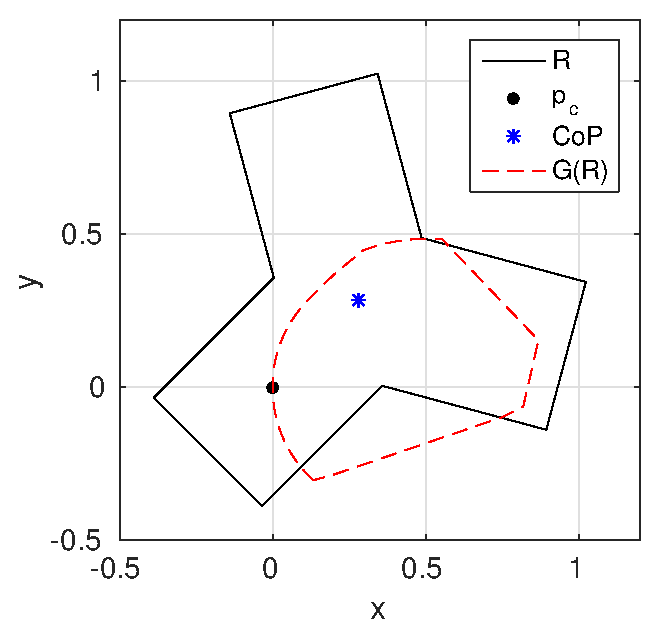
\includegraphics[width=0.7\linewidth]{fig/CoP_boundary}
      \caption{$\conv G(R) \cap \{z=0\}$}
    \end{figure}
  \end{columns}
\end{frame}

\begin{frame}{Tighter Bounds}
  \begin{columns}[T,onlytextwidth]
    \column{0.5\textwidth}
    \begin{list}{}{
        \setlength{\leftmargin}{0pt}
        \setlength{\labelwidth}{0pt}
      }
    \item Feasibility test as a linear program
      \begin{equation*}
        \begin{aligned}
          & \underset{\mathbf{p}}{\text{minimize}}
          & & \mathbf{0} \\
          & \text{subject to}
          & & G(R)\mathbf{p} = [x_0,y_0,0]^T,\\%\; \mathbf{1}\cdot\mathbf{p} = 1, \\
          & & & \mathbf{1}\cdot\mathbf{p} = 1,\; L \leq \mathbf{p} \leq U
        \end{aligned} \label{eq:lin-prog-PiCH}
      \end{equation*}\vspace{5mm}
    \item Setting $L$, $U$ controls range of pressures
      $\mathbf{p}$
    \item Can make bounds arbitrarily tight...
    \end{list}
    % \begin{itemize}
    % \item Setting $L$, $U$ controls range of pressures
    %   $\mathbf{p}$
    % \item Can make bounds arbitrarily tight...
    % \end{itemize}
    \column{0.475\textwidth}
    \begin{figure}[t]
      \centering
      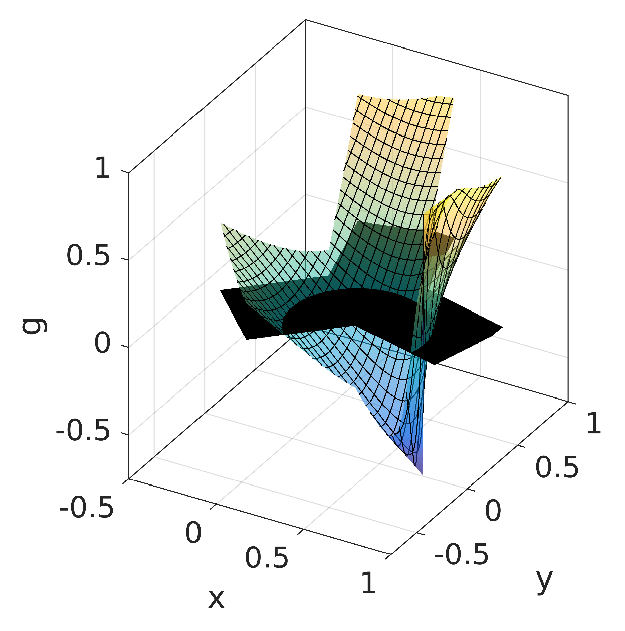
\includegraphics[width=0.7\linewidth]{fig/moment_hull_2}
      \caption{Frictional moment surface $G(R)$}
    \end{figure}
  \end{columns}
\end{frame}

\begin{frame}{Planning Robotic Pulling}
  \begin{columns}[T,onlytextwidth]
    \column{0.5\textwidth}
    \begin{list}{}{
        \setlength{\leftmargin}{0pt}
        \setlength{\labelwidth}{0pt}
      }
    \item Controls (heading + direction)
      \begin{equation*}
        u_i = [d_i, \phi_i]
      \end{equation*}
    \item DDP Dynamics
      \begin{align*}
        x_{i+1} &= x_i + d_i\cdot\cos(\phi_i) \\
        y_{i+1} &= y_i + d_i\cdot\sin(\phi_i)\\
        u_{i+1} &= u_i + d_i\cdot\hat{\alpha}(u_i - \phi_i + \pi) \\
        \ell_{i+1} &= \ell_i + d_i\cdot\hat{\beta}(\ell_i - \phi_i + \pi)\\
        h_{i+1} &= h_i + d_i.
      \end{align*}
    % \item Initialize with Dubin's paths
    \end{list}
    \column{0.5\textwidth}
    \begin{list}{}{
        \setlength{\leftmargin}{0pt}
        \setlength{\labelwidth}{0pt}
      }
    \item Loss Function
      \begin{align*}
        \mathcal{L}_F(\mathbf{x}_N,h_N) &= \mathbf{k}^T\mathcal{L}_{\bm{\delta}}(\mathbf{x}_N-\mathbf{x}_F) + \lambda h_N^2\\
        \mathcal{L}_{\delta}(a) &= \sqrt{a^2+\delta^2}-\delta
      \end{align*}
    \end{list}
    \begin{figure}
      \begin{center}
        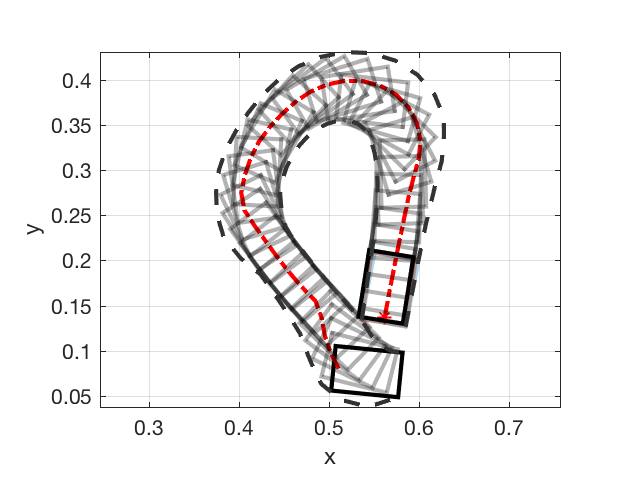
\includegraphics[width=0.8\linewidth]{fig/trajectory_2.eps}
      \end{center}
      \caption{Example trajectory in red}
      % \label{fig:trajectory}
    \end{figure}
  \end{columns}
\end{frame}

\section{Experiments}

\begin{frame}{Bounds Comparisons}
  \begin{columns}[c,onlytextwidth]
    \column{0.5\textwidth}

    \begin{list}{}{
        \setlength{\leftmargin}{0pt}
        \setlength{\labelwidth}{0pt}
        \setlength{\labelsep}{0pt}
      }
    \item Objects:
      \begin{align*}
        &\text{MIT Pushing Dataset}\\
        &\text{2/3/4-pods}
      \end{align*}
    \item Setup:
    \end{list}
    \begin{itemize}
    \item Object set 90$^\circ$
    \item Pull right until CoP converges to 1$^\circ$
    \end{itemize}

    \column{0.5\textwidth}
    \begin{figure}
      \centering
      \def\iangle{90} % Angle of the inclined plane
      \begin{tikzpicture}[
        scale=1.0, every node/.style={scale=1.0},
        force/.style={>=latex,draw=black,fill=black},
        axis/.style={densely dashed,draw=gray,font=\small},
        ]
        \fill[draw=black,fill=blue!10,thin,rotate=\iangle] (-0.3,-0.5) rectangle (2.0,.5);
        \draw[rotate=\iangle] (-0.1,0) ++(1,0) circle[radius=2.4pt] node[cross] {};
        \draw[rotate=\iangle] (-0.1,0) ++(1,0) node[above right] {\tiny CoP};
        % \draw [->,line width=1pt,rotate=-62.5] (0,0) ++(0,1) arc (90:30:1.0) node[right] {$\omega$};
        {[axis,->]
          \draw (0,0) -- (2.5,0) node[right] {$x$};
          % \draw (0,0) -- (0,2.5) node[above] {$y$};
        }
        {[force,->]
          \draw (0,0) -- ++(1.5,0) node[below right] {$\mathbf{v}$};
        }
        \fill (0,0) circle [radius=1.pt];
        % \fill (1.2207,0) circle [radius=1.pt] node[below right] {$x_{\text{\tiny IC}}$};

      \end{tikzpicture}
      % \caption{Motion of a press-pulled slider.}
      % \BB{Define variables and provide a short explanation of the figure.}}
      % \label{fig:presspull-motion}
    \end{figure}

  \end{columns}  
\end{frame}

\begin{frame}{Bounds Comparisons}
\begin{table}[t]
  \begin{center}
      \begin{tabular}[c]{cccc}
        \toprule
        & Exact & Exact-50\% & Peshkin \\
        \midrule
        MIT & $\begin{matrix}0.670\\0.172\end{matrix} \begin{matrix}\pm\\\pm\end{matrix} \begin{matrix}0.141\\ 0.047\end{matrix}$ & $\begin{matrix}\mathbf{0.362}\\\mathbf{0.243}\end{matrix} \begin{matrix}\pm\\\pm\end{matrix} \begin{matrix}0.073\\ 0.053\end{matrix}$ & $\begin{matrix}1.354\\0.162\end{matrix} \begin{matrix}\pm\\\pm\end{matrix} \begin{matrix}0.501\\ 0.041\end{matrix}$ \\
        \midrule
        Bipod & $\begin{matrix}0.762\\0.516\end{matrix} \begin{matrix}\pm\\\pm\end{matrix} \begin{matrix}0.210\\ 0.218\end{matrix}$ & $\begin{matrix}\mathbf{0.692}\\\mathbf{0.574}\end{matrix} \begin{matrix}\pm\\\pm\end{matrix} \begin{matrix}0.213\\ 0.216\end{matrix}$ & $\begin{matrix}0.899\\0.273\end{matrix} \begin{matrix}\pm\\\pm\end{matrix} \begin{matrix}0.239\\0.095\end{matrix}$ \\
        \midrule
        Tripod & $\begin{matrix}0.765\\0.522\end{matrix} \begin{matrix}\pm\\\pm\end{matrix} \begin{matrix}0.133\\ 0.162\end{matrix}$ & $\begin{matrix}\mathbf{0.688}\\\mathbf{0.576}\end{matrix} \begin{matrix}\pm\\\pm\end{matrix} \begin{matrix}0.143\\ 0.157\end{matrix}$ & $\begin{matrix}1.180\\0.340\end{matrix} \begin{matrix}\pm\\\pm\end{matrix} \begin{matrix}0.244\\0.108\end{matrix}$ \\
        \midrule
        Quadrapod & $\begin{matrix}0.880\\0.417\end{matrix} \begin{matrix}\pm\\\pm\end{matrix} \begin{matrix}0.120\\ 0.099\end{matrix}$ & $\begin{matrix}\mathbf{0.749}\\\mathbf{0.489}\end{matrix} \begin{matrix}\pm\\\pm\end{matrix} \begin{matrix}0.114\\ 0.098\end{matrix}$ & $\begin{matrix}1.207\\0.329\end{matrix} \begin{matrix}\pm\\\pm\end{matrix} \begin{matrix}0.235\\0.096\end{matrix}$ \\
        \bottomrule
      \end{tabular}
  \end{center}
  \caption{Distance-to-convergence (in meters). Top and bottom values corr. upper and lower angular velocity bounds.}
  \label{table:convergence-distance}
\end{table}
\end{frame}

\begin{frame}{Real World Pulling (Setup)}
  \begin{figure}
    \centering
    \includegraphics[width=\columnwidth]{fig/hardware.png}
    \caption{Hardware setup for robotic pulling experiments.}
    \label{fig:hardware}
  \end{figure}
\end{frame}

\begin{frame}{Real World Pulling}
  \begin{columns}[c,onlytextwidth]
    \column{0.5\textwidth}

    \begin{list}{}{
        \setlength{\leftmargin}{0pt}
        \setlength{\labelwidth}{0pt}
        \setlength{\labelsep}{0pt}
      }
    \item abs pos error: 
      \[4.00mm \pm 3.02mm\]
    \item abs ang error: 
      \[4.35^\circ  \pm 3.14^\circ\]
    \item failures:
      \[\text{4/80 runs - no valid plans}\]
    \end{list}

    \column{0.5\textwidth}

    \begin{figure}
      \begin{center}
        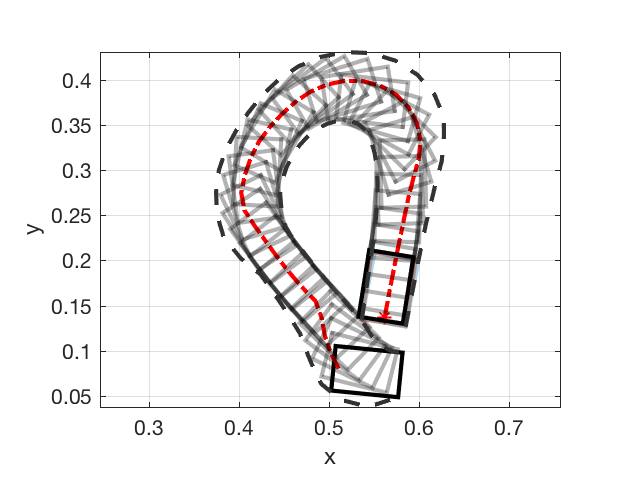
\includegraphics[width=\columnwidth]{fig/trajectory_2.eps}
      \end{center}
      \caption{Measure pulling poses and swept volume of bounds}
      % \label{fig:trajectory}
    \end{figure}

  \end{columns}
\end{frame}

% \begin{frame}{Real World Pulling}
%   \centering
%   \includemedia[
%   activate=onclick,
%   width=0.75\textwidth,
%   addresource=rss2017.mp4,
%   flashvars={%
%     source=rss2017.mp4% same path as in addresource!
%     % &autoPlay=true%    % optional configuration
%     % &loop=true%        % variables
%   }]{Pulling example on real system}{VPlayer.swf}
% \end{frame}

\begin{frame}[standout]
  Questions?
\end{frame}

\appendix

\begin{frame}[fragile]{Backup slides}
  Sometimes, it is useful to add slides at the end of your presentation to
  refer to during audience questions.

  The best way to do this is to include the \verb|appendixnumberbeamer|
  package in your preamble and call \verb|\appendix| before your backup slides.

  \themename will automatically turn off slide numbering and progress bars for
  slides in the appendix.
\end{frame}

\begin{frame}[allowframebreaks]{References}

  \bibliography{references}
  \bibliographystyle{abbrv}

\end{frame}

\end{document}
